\section{Erwin Transformer}
\label{section:erwin}

\begin{figure*}[t]
    \centering
    \small
    \hspace*{-1.2cm}
    \subfigure[Alignment stage]{
    \begin{minipage}[t]{0.24\linewidth}
    \centering
      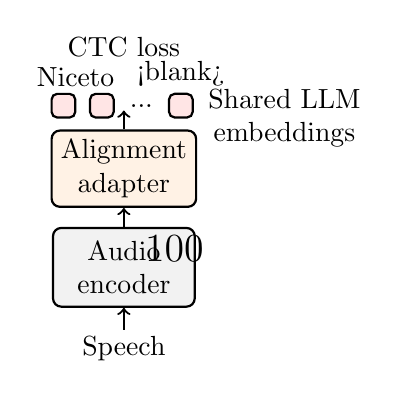
\begin{tikzpicture} [scale=0.8]
        \node(ae) at (0,0) [rectangle, draw=black, fill=gray!10, rounded corners=3pt, thick, minimum width=1.8cm,minimum height=1cm,align=center] {Audio\\encoder};
        \node(freeze) at ([xshift=0.8cm,yshift=0.3cm]ae.center) [rectangle, align=center] {\Large{\ding{100}}};
        \node(fb) at ([yshift=-0.3cm]ae.south) [rectangle, align=center,anchor=north] {Speech};
        \node(aa) at ([yshift=0.3cm]ae.north) [rectangle, draw=black, fill=orange!10, rounded corners=3pt, thick, minimum width=1.8cm,minimum height=0.5cm,align=center,anchor=south] {Alignment\\adapter};
        
        \node(f1) at ([yshift=1.0cm]aa.west) [rectangle, draw=black, fill=red!10, rounded corners=2pt, thick, minimum width=0.3cm, minimum height=0.3cm,align=center,anchor=west] {};
        \node(f2) at ([xshift=0.2cm]f1.east) [rectangle, draw=black, fill=red!10, rounded corners=2pt, thick, minimum width=0.3cm, minimum height=0.3cm,align=center,anchor=west] {};
        \node(f3) at ([xshift=0.075cm]f2.east) [rectangle, draw=white,  thick, align=center,anchor=west] {...};
        \node(f4) at ([xshift=0.075cm]f3.east) [rectangle, draw=black, fill=red!10, rounded corners=2pt, thick, minimum width=0.3cm, minimum height=0.3cm,align=center,anchor=west] {};
        \node(t1) at ([yshift=-0.05cm]f1.north) [rectangle, align=center,anchor=south] {Nice};
        \node(t2) at ([yshift=-0.05cm]f2.north) [rectangle, align=center,anchor=south] {to};
        \node(t4) at ([yshift=-0.05cm]f4.north) [rectangle, align=center,anchor=south] {<blank>};
        \node(se) at ([xshift=0.075cm,yshift=-0.2cm]f4.east) [rectangle, align=center,anchor=west] {Shared LLM\\embeddings};
        \node(ctc) at ([yshift=1.0cm]aa.north) [rectangle, rounded corners=3pt, thick, align=center,anchor=south] {CTC loss};

        
        \draw[->,thick]([yshift=-0.05cm]fb.north)--(ae.south);
        \draw[->,thick](ae.north)--(aa.south);
        \draw[->,thick](aa.north)--([yshift=0.3cm]aa.north);

        
      \end{tikzpicture}
    \end{minipage}
    }
    \subfigure[Shrinking stage]{
    \begin{minipage}[t]{0.45\linewidth}
    \centering
    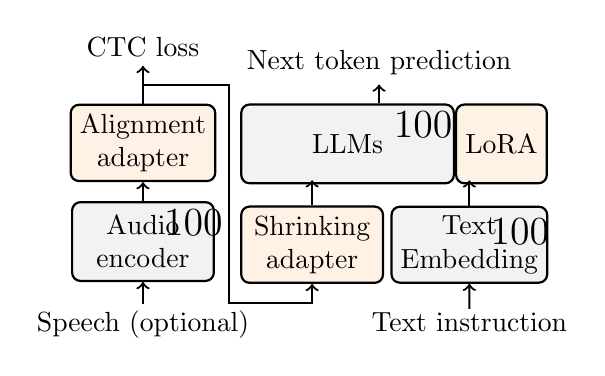
\begin{tikzpicture} [scale=0.8]
        \node(ae) at (0,0) [rectangle, draw=black, fill=gray!10, rounded corners=3pt, thick, minimum width=1.8cm,minimum height=1cm,align=center] {Audio\\encoder};
        \node(freeze) at ([xshift=0.8cm,yshift=0.3cm]ae.center) [rectangle, align=center] {\Large{\ding{100}}};
        \node(fb) at ([yshift=-0.3cm]ae.south) [rectangle, align=center,anchor=north] {Speech (optional)};
        \node(aa) at ([yshift=0.3cm]ae.north) [rectangle, draw=black, fill=orange!10, rounded corners=3pt, thick, minimum width=1.8cm,minimum height=0.5cm,align=center,anchor=south] {Alignment\\adapter};
        \node(ctc) at ([yshift=0.6cm]aa.north) [rectangle,align=center,anchor=south] {CTC loss};
        \node(sa) at ([xshift=0.4cm,yshift=-0.05cm]ae.east) [rectangle, draw=black, fill=orange!10, rounded corners=3pt, thick, minimum width=1.8cm,minimum height=0.5cm,align=center,anchor=west] {Shrinking\\adapter};
        \node(llm) at ([yshift=1.6cm]sa.west) [rectangle, draw=black, fill=gray!10, rounded corners=3pt, thick, minimum width=2.7cm,minimum height=1.0cm,align=center,anchor=west] {LLMs};
        \node(lora) at (llm.east) [rectangle, draw=black, fill=orange!10, rounded corners=3pt, thick, minimum width=1.0cm,minimum height=1.0cm,align=center,anchor=west] {LoRA};
        \node(te) at ([xshift=0.1cm]sa.east) [rectangle, draw=black, fill=gray!10, rounded corners=3pt, thick, minimum width=1.8cm,minimum height=0.5cm,align=center,anchor=west] {Text\\Embedding};
        \node(freeze3) at ([xshift=0.8cm,yshift=0.2cm]te.center) [rectangle, align=center] {\Large{\ding{100}}};
        \node(ti) at ([yshift=-0.3cm]te.south) [rectangle, align=center,anchor=north] {Text instruction};
        \node(freeze2) at ([xshift=1.2cm,yshift=0.3cm]llm.center) [rectangle, align=center] {\Large{\ding{100}}};
        \node(loss) at ([xshift=0.5cm, yshift=0.3cm]llm.north) [rectangle, align=center,anchor=south] {Next token prediction};

        
        \draw[->,thick]([yshift=-0.05cm]fb.north)--(ae.south);
        \draw[->,thick](ae.north)--(aa.south);
        \draw[->,thick](aa.north)--(ctc.south);
        \draw[->,thick](sa.north)--([yshift=0.4cm]sa.north);
        \draw[->,thick](te.north)--([yshift=0.4cm]te.north);
        \draw[->,thick]([yshift=-0.3cm]loss.south)--(loss.south);
        \draw[->,thick]([yshift=-0.1cm]ti.north)--(te.south);

        \draw[->,thick](aa.north)--([yshift=0.3cm]aa.north)--([xshift=0.2cm, yshift=0.3cm]aa.north -| aa.east)--([xshift=0.2cm, yshift=-0.3cm]sa.south -| aa.east)--([yshift=-0.3cm]sa.south)--(sa.south);
      \end{tikzpicture}
    \end{minipage}
    }
    \subfigure[SFT stage]{
    \begin{minipage}[t]{0.20\linewidth}
    \centering
    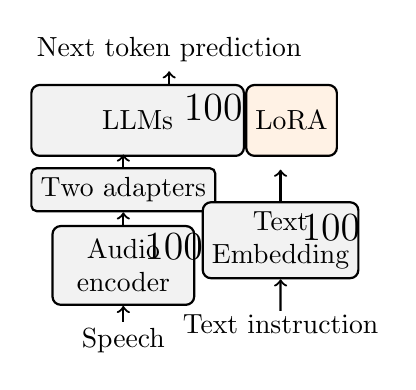
\begin{tikzpicture} [scale=0.8]
        \node(ae) at (0,0) [rectangle, draw=black, fill=gray!10, rounded corners=3pt, thick, minimum width=1.8cm,minimum height=1cm,align=center] {Audio\\encoder};
        \node(freeze) at ([xshift=0.8cm,yshift=0.3cm]ae.center) [rectangle, align=center] {\Large{\ding{100}}};
        \node(fb) at ([yshift=-0.2cm]ae.south) [rectangle, align=center,anchor=north] {Speech};
        \node(aa) at ([yshift=0.2cm]ae.north) [rectangle, draw=black, fill=gray!10, rounded corners=2pt, thick, minimum width=1.8cm,minimum height=0.5cm,align=center,anchor=south] {Two adapters};
        
        \node(llm) at ([yshift=1.1cm]aa.west) [rectangle, draw=black, fill=gray!10, rounded corners=3pt, thick, minimum width=2.7cm,minimum height=0.9cm,align=center,anchor=west] {LLMs};
        \node(lora) at (llm.east) [rectangle, draw=black, fill=orange!10, rounded corners=3pt, thick, minimum width=0.9cm,minimum height=0.9cm,align=center,anchor=west] {LoRA};
        \node(te) at ([xshift=0.1cm,yshift=0.4cm]ae.east) [rectangle, draw=black, fill=gray!10, rounded corners=3pt, thick, minimum width=1.8cm,minimum height=0.5cm,align=center,anchor=west] {Text\\Embedding};
        \node(freeze3) at ([xshift=0.8cm,yshift=0.2cm]te.center) [rectangle, align=center] {\Large{\ding{100}}};
        \node(ti) at ([yshift=-0.4cm]te.south) [rectangle, align=center,anchor=north] {Text instruction};
        \node(freeze2) at ([xshift=1.2cm,yshift=0.2cm]llm.center) [rectangle, align=center] {\Large{\ding{100}}};
        \node(loss) at ([xshift=0.5cm, yshift=0.2cm]llm.north) [rectangle, align=center,anchor=south] {Next token prediction};
       
        \draw[->,thick]([yshift=-0.05cm]fb.north)--(ae.south);
        \draw[->,thick](ae.north)--(aa.south);
        \draw[->,thick](aa.north)--([yshift=0.2cm]aa.north);
        \draw[->,thick](te.north)--([yshift=0.5cm]te.north);
        \draw[->,thick]([yshift=-0.2cm]loss.south)--(loss.south);
        \draw[->,thick]([yshift=-0.1cm]ti.north)--(te.south);
        
      \end{tikzpicture}
    \end{minipage}
    }
      \caption{Training progress of Soundwave. The gray modules are frozen while the orange modules are updated.}
      \label{architecture}
  \end{figure*}

  
Following the notation from the background Section \ref{section:ball_tree}, we consider a point cloud $P = \{ \mathbf{p}_1, ..., \mathbf{p}_n\} \subset \mathbb{R}^d$. Additionally, each point is now endowed with a feature vector yielding a feature set $X = \{ \mathbf{x}_1, ..., \mathbf{x}_n \} \subset \mathbb{R}^C$.

On top of the point cloud, we build a ball tree $T = \{ L_0, ..., L_m\}$. We initialize $L_\mathrm{leaf} := L_0$ to denote the current finest level of the tree. As each leaf node contains a single point, it inherits its feature vector:
\begin{equation}
    X_{\mathrm{leaf}} = \{ \mathbf{x}_B = \mathbf{x}_i \mid B = \{\mathbf{p}_i\} \in L_\mathrm{leaf} \}
\end{equation}

\subsection{Ball tree attention} \label{sec:ball-tree-attn}
\paragraph{Ball attention}
For each ball attention operator, we specify a level $k$ of the ball tree where each ball $B \in L_k$ contains $2^k$ leaf nodes. The choice of $k$ presents a trade-off: larger balls capture longer-range dependencies, while smaller balls are more resource-efficient. For each ball $B \in L_k$, we collect the leaf nodes within B
\begin{equation}
\mathrm{leaves}_B = \{ B' \in L_\mathrm{leaf} \mid B' \subset B \}
\end{equation}
along with their features from $X_\mathrm{leaf}$
\begin{equation}
    X_B = \{ \mathbf{x}_{B'} \in X_\mathrm{leaf} \mid B' \in \mathrm{leaves}_B \}
\end{equation}
We then compute self-attention independently on each ball\footnote{For any set of vectors $X$, we abuse notation by treating $X$ as a matrix with vectors as its rows.}:
\begin{equation}
\label{eq:ball_attention}
    X'_B = \mathrm{BAtt}(X_B):= \mathrm{Att}(X_B \mathbf{W}_q, X_B \mathbf{W}_k, X_B \mathbf{W}_v)
\end{equation}
where weights are shared between balls and the output $X'_B$ maintains row correspondence with $X_B$. 

\paragraph{Computational cost}
As attention is computed independently for each ball $B \in L_k$, the computational cost is reduced from quadratic to linear. Precisely, for ball attention, the complexity is $\mathcal{O}(|B|^2 \cdot \frac{n}{|B|})$, i.e. quadratic in the ball size and linear in the number of balls:
\begin{figure}[H]
\centering
    \begin{tikzpicture}
        \node[anchor=south west,inner sep=0] (image) at (0,0) 
            {\includegraphics[width=0.7\linewidth]{figures/raw/attention_comp.pdf}};
        
        \begin{scope}[x={(image.south east)},y={(image.north west)}]
            \node[color=black] at (0.2,1.2) {Attention $\mathcal{O}(n^2)$};
        \end{scope}

        \begin{scope}[x={(image.south east)},y={(image.north west)}]
            \node[color=black] at (0.8,1.2) {Ball Attention $\mathcal{O}(n)$};
        \end{scope}
    \end{tikzpicture}
    \caption{For highlighted points, standard attention computes interactions with all other points in the point cloud, while ball attention only considers points within their balls.}
    \label{fig:attention_comp}
\end{figure}


\paragraph{Positional encoding}
We introduce positional information to the attention layer in two ways. First, we augment the features of leaf nodes with their relative positions with respect to the ball's center of mass (relative position embedding):
\begin{equation}
\label{eq:rpe}
    \text{RPE}: \qquad X_B = X_B + (P_B - \mathbf{c}_B) \mathbf{W}_{\mathrm{pos}}
\end{equation}
where $P_B$ contains positions of leaf nodes, $\mathbf{c}_B$ is the center of mass, and $\mathbf{W}_{\mathrm{pos}}$ is a learnable projection. This allows the layer to incorporate geometric structure within each ball. 

Second, we introduce a distance-based attention bias:
\begin{equation}
\label{eq:bias}
    \mathcal{B}_{B} = - \sigma^2 ||\mathbf{c}_{B'} - \mathbf{c}_{B''}||_2, \quad B', B'' \in \mathrm{leaves}_B
\end{equation}
with a learnable parameter $\sigma \in \mathbb{R}$ \cite{Wessels2024GroundingCR}. The term decays rapidly as the distance between two nodes increases which enforces locality and helps to mitigate potential artifacts from the tree building, particularly in cases where distant points are grouped together.

\paragraph{Cross-ball connection}
To increase the receptive field of our attention operator, we implement cross-ball connections inspired by the shifted window approach in Swin Transformer \cite{Liu2021SwinTH}. There, patches are displaced diagonally by half their size to obtain two different image paTreertitioning configurations. This operation can be equivalently interpreted as keeping the patches fixed while sliding the image itself. 

Following this interpretation, we rotate the point cloud and construct the second ball tree $T_\mathrm{rot} = \{ L_0^{\mathrm{rot}}, ..., L_m^{\mathrm{rot}} \}$ which induces a permutation $\pi^{\mathrm{rot}}$ of leaf nodes (see Fig. \ref{fig:overview}, center). We can then compute ball attention on the rotated configuration by first permuting the features according to $\pi^{\mathrm{rot}}$, applying attention, and then permuting back:

\begin{equation}
\label{eq:rot_ball_attention}
    X'_B = \pi^{-1}_{\mathrm{rot}} \left( \mathrm{BAtt}\left(\pi_{\mathrm{rot}} \left( X_B \right) \right) \right)
\end{equation}

By alternating between the original and rotated configurations in consecutive layers, we ensure the interaction between leaf nodes in otherwise separated balls.

\paragraph{Tree coarsening/refinement}
For larger systems, we are interested in coarser representations to capture features at larger scales. The coarsening operation allows us to hierarchically aggregate information by pooling leaf nodes to the centers of containing balls at $l$ levels higher (see Fig. \ref{fig:overview}, top, $l=1$). Suppose the leaf level is $k$. For every ball $B \in L_{k+l}$, we concatenate features of all interior leaf nodes along with their relative positions with respect to $\mathbf{c}_B$ and project them to a higher-dimensional representation:
\vspace{-3pt}
\begin{equation}
\vspace{-2pt}
   \mathbf{x}_B = \left( \bigoplus_{B' \in \mathrm{leaves}_B} \left[ \mathbf{x}_{B'}, \mathbf{c}_{B'} - \mathbf{c}_{B} \right] \right) \mathbf{W}_c
\end{equation}
where $\bigoplus$ denotes leaf-wise concatenation, and $\mathbf{W}_c \in \mathbb{R}^{C' \times 2^l(C + d)}$ is a learnable projection that increases the feature dimension to maintain expressivity. After coarsening, balls at level $k+l$ become the new leaf nodes, $L_\mathrm{leaf} := L_{k+l}$, with features $X_\mathrm{leaf} := \{\mathbf{x}_B \mid B \in L_{k+l}\}$. To highlight the simplicity of our method, we provide the pseudocode\footnote{We use \texttt{einops} \cite{rogozhnikov2022einops} primitives.}:

\begin{tikzpicture}
    \begin{scope}[x={(image.south east)},y={(image.north west)}]
        \node[draw=gray!30, fill=gray!5, rounded corners, 
              inner sep=5pt,
              text width=0.95\linewidth,
              align=left, 
              anchor=center,
              font=\ttfamily\fontsize{7.25pt}{7.5pt}\selectfont] (code) at (0.468, 0.135) {
        \color[HTML]{595959}{\# coarsening ball tree} \\
        \color{black}
        x = \textcolor[HTML]{9c4461}{rearrange}([x, rel.pos], \textcolor{orange}{"(n $2^l$) d $\rightarrow$ n ($2^l$ d)"}) @ $W_c$  \\
        pos = \textcolor[HTML]{9c4461}{reduce}(pos, \textcolor{orange}{"(n $2^l$) d $\rightarrow$ n d"}, \textcolor{orange}{"mean"}) \\
        };
    \end{scope}
\end{tikzpicture}

The inverse operation, refinement, allocates information from a coarse representation back to finer scales. More precisely, for a ball $B \in L_k$, its features are distributed back to the nodes at level $L_{k-l}$ contained within $B$ as
\vspace{-1pt}
\begin{equation}
\vspace{-1pt}
  \{\mathbf{x}_{B'} \mid B' \in L_{k-l}\} = \left[\mathbf{x}_B, P_B - \mathbf{c}_B \right] \: \mathbf{W}_r
\end{equation}
where $P_B$ contains positions of all nodes at level $k-l$ within ball $B$ with center of mass $\mathbf{c}_B$, and $\mathbf{W}_r \in \mathbb{R}^{2^lC \times (C'+d)}$ is a learnable projection. After refinement, $L_\mathrm{leaf}$ and $X_\mathrm{leaf}$ are updated accordingly. In pseudocode:

\begin{tikzpicture}
    \begin{scope}[x={(image.south east)},y={(image.north west)}]
        \node[draw=gray!30, fill=gray!5, rounded corners, 
              inner sep=5pt,
              text width=0.95\linewidth,
              align=left, 
              anchor=center,
              font=\ttfamily\fontsize{7.25pt}{7.5pt}\selectfont] (code) at (0.468, 0.135) {
        \color[HTML]{595959}{\# refining ball tree} \\
        \color{black}
        x = [\textcolor[HTML]{9c4461}{rearrange}(x, \textcolor{orange}{"n ($2^l$ d) $\rightarrow$ (n $2^l$) d"}), rel.pos] @ $W_r$
        };
    \end{scope}
\end{tikzpicture}


\subsection{Model architecture}
\vspace{-2pt}
We are now ready to describe the details of the main model to which we refer as \emph{Erwin}\footnote{We pay homage to Swin Transformer as our model based on rotating windows instead of sliding, hence Rwin $\rightarrow$ Erwin.} (see Fig. \ref{fig:overview}) - a hierarchical transformer operating on ball trees.

\vspace{-8pt}
\paragraph{Embedding}
At the embedding phase, we first construct a ball tree on top of the input point cloud and pad the leaf layer to complete the tree, as described in Section \ref{section:ball_tree}. To capture local geometric features, we employ a small-scale MPNN, which is conceptually similar to PointTransformer's embedding module using sparse convolution. When input connectivity is not provided (e.g. mesh), we utilize the ball tree structure for a fast nearest neighbor search.

\vspace{-8pt}
\paragraph{ErwinBlock}
The core building block of Erwin follows a standard pre-norm transformer structure: LayerNorm followed by ball attention with a residual connection, and a SwiGLU feed-forward network \cite{Shazeer2020GLUVI}. For the ball attention, the size $2^k$ of partitions is a hyperparameter. To ensure cross-ball interaction, we alternate between the original and rotated ball tree configurations, using an even number of blocks per \textbf{ErwinLayer} in our experiments.

\vspace{-8pt}
\paragraph{Overall architecture}
Following a UNet structure \cite{Ronneberger2015UNetCN, Wu2023PointTV}, Erwin processes features at multiple scales through encoder and decoder paths (Fig. \ref{fig:overview}, right). The encoder progressively coarsens the ball tree while increasing feature dimensionality to maintain expressivity. The coarsening factor is a hyperparameter that takes values that are powers of $2$. At the decoder stage, the representation is refined back to the original resolution, with skip connections from corresponding encoder levels enabling multi-scale feature integration.



